
\documentclass[
12pt,
a4paper,
pdftex,
czech,
titlepage
]{report}
\usepackage{hyperref}
\usepackage[czech]{babel}
\usepackage[table]{xcolor}
\usepackage{array}
\usepackage[utf8]{inputenc}
\usepackage{lmodern}
\usepackage{textcomp}
\usepackage[T1]{fontenc}
\usepackage{amsfonts}
\usepackage{titlesec}
\usepackage{graphicx}
\usepackage{enumitem}
\usepackage{changepage}
\usepackage{csquotes}
\usepackage{listings}


\lstset{
  basicstyle=\small\ttfamily, % Nastaví menší písmo s pevnou šířkou
  breaklines=true,            % Povolení automatického zalamování řádků
  breakatwhitespace=true,     % Zalamování bude probíhat pouze na mezerách
  columns=fullflexible,       % Umožní lepší zalamování řádků
  frame=single,               % Ohraničí kód rámečkem
  captionpos=b,               % Umístí popisek pod kód
  numbers=left,               % Číslování řádků vlevo
  numberstyle=\tiny,          % Menší písmo pro čísla řádků
  stepnumber=1,               % Číslovat každý řádek
  tabsize=2,                  % Nastaví šířku tabulátoru na 2 mezery
  showspaces=false,           % Nezobrazovat mezery zvlášť
  showstringspaces=false,     % Nezobrazovat mezery ve stringách
  showtabs=false              % Nezobrazovat tabulátory zvlášť
}



\titleformat{\chapter}
  {\normalfont\LARGE\bfseries}{\thechapter}{1em}{}
\titlespacing*{\chapter}{0pt}{0ex plus 1ex minus .2ex}{2.0ex plus .2ex}

\begin{document}

\begin{titlepage}
	\vspace*{-2cm}
	{\centering
\includegraphics[scale=1.0]{logo.png}\par}
	\centering
	\vspace*{2cm}
	{\Large Semestrální práce z KIV/PC\par}
	\vspace{1.5cm}
	{\Huge\bfseries Nástroj pro řešení úloh lineárního programování\par}
	\vspace{2cm}

	{\Large Tomáš Vítek\par}
	{\Large A21B0316P\par}
	{\Large twitty@students.zcu.cz\par}

	\vfill

	{\Large 4.\,1.\,2025}
\end{titlepage}

\tableofcontents
\thispagestyle{empty}
\clearpage

\chapter{Zadání}
\setcounter{page}{1}

Naprogramujte v jazyce ANSI C přenositelnou \textbf{konzolovou aplikaci}, která
bude řešit úlohy lineárního programování zadané ve zjednodušeném formátu
LP.

Program bude spouštěn příkazem lp.exe2s kombinací následujících
argumentů -- výrazy v lome-ných závorkách (\textless\textgreater), resp.
hranatých závorkách ({[}{]}) označují povinné, resp. nepovinné argumenty:

\begin{itemize}[label={}]
\item <input-file>
\hspace{1.5cm} \begin{minipage}[t]{0.6\textwidth}  Soubor s popisem úlohy ve formátu LP.
V případě, že uživatel zadá neexistu- jící soubor, program vypíše
chybové hlášení \texttt{"Input file not found!{\textbackslash{}}n}" a vrátí
hodnotu 1.
\end{minipage}

\item -o <path>
\hspace{1.8cm} \begin{minipage}[t]{0.6\textwidth} Výstupní soubor s řešením úlohy. Pokud
umístění neexistuje, bude vypsáno hlášení \texttt{"Invalid output
destination!\emph{\textbackslash{}}n"} a program skončí s návrato-vou
hodnotou 2. V případě, že uživatel tento přepínač nezadá, bude výsledek
optimalizace vypsán na obrazovku. Do tohoto souboru neuvádějte chybová
hlášení.
\end{minipage}

\item --output <path>
\hspace{0.7cm} \begin{minipage}[t]{0.6\textwidth} Stejné jako v případě přepínače
-o. Použití obou přepínačů -o a -\/-output není chybou, program pak bude
akceptovat poslední zadanou hodnotu.
\end{minipage}
\end{itemize}

V případě nalezení konečného optimálního řešení úlohy program vrátí
hodnotu EXIT\_SUCCESS. Chybové stavy týkající se zpracování vstupních
souborů nebo samotného algoritmu optimalizace jsou popsány v dalších
sekcích.
\\

Hotovou práci odevzdejte v jediném archivu typu ZIP prostřednictvím automatického odevzdávacího a validačního systému. Postupujte podle instrukcí uvedených na webu předmětu. Archiv nechť
obsahuje všechny zdrojové soubory potřebné k přeložení programu, \textbf{Makefile} pro Windows i Linux
(pro překlad v Linuxu připravte soubor pojmenovaný \texttt{Makefile} a pro Windows Makefile.win)
a dokumentaci ve formátu PDF vytvořenou v typografickém systému \TeX (\LaTeX). Bude-li některá
z částí chybět, kontrolní skript Vaši práci odmítne.

\section*{Specifikace vyhodnocovaných výrazů
}

Pro zachycení optimalizačního modelu bude program používat redukovanou a
zobecněnou verzi formátu LP. Vstupní soubory
mohou obsahovat následující sekce:

\begin{itemize}[label={}]
\item \texttt{Maximaze/Minimaze}
\hspace{1cm} \begin{minipage}[t]{0.56\textwidth}  Výraz uvozující řádek se zápisem optimalizované
účelové funkce. Pro-gram musí být schopen zpracovat standardní operátory
+, -, *, = nebo závorky (), {[}{]} a \{\}. Oproti originální verzi ovšem
nevyžadujeme, aby jednotlivé operandy a operátory byly v matematických
výrazech striktněodděleny mezerou (to platí i v ostatních sekcích
souboru). Názvy pro-měnných tedy dříve uvedené operátory a závorky
obsahovat nesmí. Při násobení není nutné použít operátor *, například
"2.5z" značí \textit{2,5 krát \emph{z}}, zatímco "z2" je pouze název proměnné.
\end{minipage}

\item \texttt{Subject To}
\hspace{2.6cm} \begin{minipage}[t]{0.56\textwidth} Sekce obsahující seznam podmínek ve formátu
\texttt{"\textless název\textgreater: \textless výraz\textgreater"}. Navíc oproti
účelové funkci mohou podmínky obsahovat porovnávacíoperátory \texttt{ \textless,
\textgreater, \textless= a \textgreater=}.
\end{minipage}

\item \texttt{Bounds}
\hspace{3.4cm} \begin{minipage}[t]{0.56\textwidth} Omezení hodnot rozhodovacích proměnných. V této sekci jsou
povoleny pouze porovnávací operátory uvedené výše.
\end{minipage}

\item \texttt{Generals}
\hspace{3cm} \begin{minipage}[t]{0.56\textwidth}   Obsahuje seznam použitých rozhodovacích proměnných oddělených
znaménkem mezery. Pokud je v souboru nalezena proměnná, která v této sekci
není uvedena, program skončí s chybovou hláškou \texttt{"Unknown
variable'\textless j\textgreater'!\emph{\textbackslash{}}n"}, kde
\texttt{\textless j\textgreater{}} je neznámá proměnná, a návratovou hodnotou 10.
Pokud sekce obsahuje nepoužitou rozhodovací proměnnou
\texttt{\textless n\textgreater}, program vypíše pouze varování \texttt{"Warning: unused
variable '\textless n\textgreater'!\emph{\textbackslash{}}n"}.
\end{minipage}


\item \texttt{End}
\hspace{4.2cm} \begin{minipage}[t]{0.56\textwidth} Uvozuje konec souboru, tzn. že se vyskytuje vždy jako poslední a
sekce uvedené za ním jsou syntaktickou chybou.
\end{minipage}


Až na návěští \texttt{End} není pořadí jednotlivých sekcí fixní. Na výskyt
neplatných operátorů, neznámých sekcí a jiných problémů program reaguje
vypsáním chybového hlášení \texttt{"Syntax error!\emph{\textbackslash{}}n"} a
skončí s návratovou hodnotou 11. Komentáře v souboru jsou uvozeny znakem
"\emph{\textbackslash{}}". Ukázku vstupního souboru si můžete
prohlédnout v konzolovém rozhraní 1 na straně 4.

\section*{Optimalizační algoritmus}

Při analýze úlohy jistě narazíte na problémy degenerovaných úloh a jiné,
které budeme pro jed-noduchost ignorovat. Algoritmus hledání optimálního
řešení úlohy lineárního programování může tedy teoreticky skončit
následovně.

\begin{enumerate}[label=\arabic*.]
\item \textbf{Nalezení konečného optimálního řešení}
V takovém případě program vypíše optimální hodnoty rozhodovacích
proměnných a skončís návratovou hodnotou \texttt{EXIT\_SUCCESS}. Optimálních řešení může být více, s čímž
validační skript počítá.

\item \textbf{Úloha je neomezená}
Účelová funkce může nabývat libovolně velkých hodnot, aniž by porušila
některou z omezují-cích podmínek, tj. optimum je v nekonečnu. Program na
tuto skutečnost upozorní chybovým hlášením \texttt{"Objective function is
unbounded. \emph{\textbackslash{}}n"} a skončí s návratovou hodnotou 20.

\item \textbf{Neexistence přípustného řešení}
Soustava omezení nemá žádnou společnou přípustnou oblast, tj. neexistuje
žádný bod, kterýby vyhovoval všem omezením současně -- úloha je
nesplnitelná. V takovém případě program vypíše chybovou hláškou \texttt{"No
feasible solution exists.\emph{\textbackslash{}}n"} a vrátí hodnotu 21.
\end{enumerate}


\chapter{Analýza úlohy}

\section{Zadání}
Zadání úlohy vyžaduje naprogramování konzolové přenositelné aplikace v jazyce \textbf{ANSI C}. Jejím obsahem bude implementace nástroje pro řešení úloh lineárního programovní.

\section{Lineární úlohy}

Lineární úloha je matematický problém, který lze formulovat pomocí lineární funkce nebo rovnice. V těchto úlohách jsou rozhodujícími faktory proměnné, které jsou v lineární závislosti na jiných proměnných. V běžné podobě se lineární úlohy vyskytují jako optimalizační problémy, kde je cílem maximalizovat nebo minimalizovat určitou funkci (např. zisk, náklady) za podmínek (omezeních), které jsou vyjádřeny jako lineární rovnice nebo nerovnice.

\subsection*{Formulace lineární úlohy}
Obecná formulace lineární úlohy zahrnuje:
\begin{itemize}
  \item \textbf{Cílová funkce}: Funkce, kterou chceme maximalizovat nebo minimalizovat. Obvykle se vyjadřuje jako lineární kombinace proměnných, např.:
  \[
  Z = c_1 x_1 + c_2 x_2 + \dots + c_n x_n
  \]
  kde \( c_1, c_2, \dots, c_n \) jsou koeficienty, a \( x_1, x_2, \dots, x_n \) jsou rozhodovací proměnné.
  \item \textbf{Omezení}: Podmínky, které musí být splněny, jsou vyjádřeny jako soustava lineárních rovnic nebo nerovnic. Například:
  \[
  a_{11} x_1 + a_{12} x_2 + \dots + a_{1n} x_n \leq b_1
  \]
  \[
  a_{21} x_1 + a_{22} x_2 + \dots + a_{2n} x_n \geq b_2
  \]
  kde \( a_{ij} \) jsou koeficienty a \( b_1, b_2, \dots, b_m \) jsou pravé strany rovnic nebo nerovnic.
  \item \textbf{Meze}: V některých úlohách je potřeba, aby proměnné byly nezáporné, tj. \( x_1 \geq 0, x_2 \geq 0, \dots, x_n \geq 0 \).
\end{itemize}

Lineární úlohy se obvykle řeší pomocí \textbf{simplexové metody}, která je algoritmem pro hledání optimálního řešení v diskrétní množině. Existují také další metody, jako \textbf{grafické řešení} (pro úlohy se dvěma proměnnými) nebo použití specializovaných softwarových nástrojů, například \textbf{LP solvers} (linear programming solvers).

\section{Simpexový alogritmus}


Simplexový algoritmus je jedním z nejpopulárnějších a nejefektivnějších algoritmů pro řešení lineárních optimalizačních úloh. Tento algoritmus je iterativní metodou, která začíná v jednom z vrcholů konvexní množiny řešení a postupně se přesouvá k sousedním vrcholům. Proces pokračuje, dokud nenalezne optimální řešení nebo se nepotvrdí, že úloha nemá řešení. Simplexový algoritmus vždy dosáhne optimálního řešení v jednom z vrcholů, pokud existuje.

\subsection*{Princip fungování}

Simplexový algoritmus hledá optimální řešení v diskrétní množině vrcholů polyhedronu definovaného omezeními lineární úlohy. Každý krok algoritmu je zaměřen na zlepšení hodnoty cílové funkce, dokud není dosaženo optimálního řešení.

Algoritmus pracuje s tzv. \textbf{simplexovou tabulkou}, která je sestavena z koeficientů cílové funkce, omezení a proměnných. Na každém kroku algoritmus provádí výpočty, které vedou k pohybu mezi vrcholy polyhedronu směrem k optimálnímu bodu.

\subsection*{Kroky simplexového algoritmu}

\begin{itemize}
    \item \textbf{Inicializace}: Nejprve se sestaví počáteční simplexová tabulka, která obsahuje informace o koeficientech lineární úlohy. Tato tabulka představuje počáteční řešení, které není nutně optimální.
    
    \item \textbf{Výběr vstupní proměnné}: Zvolí se proměnná, která nejvíce zlepšuje hodnotu cílové funkce. Tato proměnná je přidána do báze.
    
    \item \textbf{Výběr výstupní proměnné}: Určí se proměnná, která musí být odstraněna z báze, aby byla zachována konzistence s omezeními. Tento krok zaručuje, že zůstáváme v prostoru povolených řešení.
    
    \item \textbf{Aktualizace simplexové tabulky}: Po výběru proměnných se aktualizují hodnoty v simplexové tabulce podle pravidel algoritmu. Tato tabulka se používá pro výpočet nových hodnot proměnných v dalším kroku.
    
    \item \textbf{Opakování}: Tento proces se opakuje, dokud všechny koeficienty v řádku cílové funkce nebudou nenegativní, což indikuje dosažení optimálního řešení.
\end{itemize}

\subsection*{Výhody a nevýhody}

Simplexový algoritmus je velmi efektivní v praxi a obvykle najde optimální řešení v relativně krátkém čase. I když teoreticky může mít exponenciální složitost, v reálných úlohách je výkon obvykle velmi dobrý. Nicméně, v extrémních případech může algoritmus selhat a zůstat u suboptimálních řešení.

Jedním z možných problémů je, že simplexový algoritmus může někdy projít cyklem, což znamená, že se vrátí zpět na stejný bod bez pokroku. Tento problém je možné vyřešit pomocí různých modifikací, jako je pravidlo Bland nebo použití \textit{dual simplex method}.
ss
\chapter{Popis implementace}

Projekt je implementován v jazyce \textit{ANSI C} za použití standartních knihoven \textit{<stdio.h>, <stdlib.h>, <ctype.h>, <limits.h>} a \textit{<string.h>}.
Projekt je rozdělen do jedenácti hlavičkových a dvanácti \textit{.c} souborů. Každý \textit{.c} soubor má s výjimkou \textit{Main.c} souboru vlastní stejnojmený .h soubor.

V souborech \textit{Description, Matrix, Bounds, Logger a Result} se nachází implementace stejnojmenných struktur a funkcí k jejich alokaci, inicializaci, měnění obsahu jejich hodnot, deinicializaci a dealokaci. 

Soubory \textit{FileReader} obsahují implementaci načítání vstupních údajů od uživatele, ať už z příkazového řádku, tak ze souboru.
Výpis informací do souborů a do příkazového řádku obsahují soubory \textit{ResultWriter}.

\textit{Global} slouží k deklaraci a inicializaci globálních proměnných dostupných v souborech \textit{Main} a \textit{Exit}. Jinde v kódu se tyto struktury nepoužívají a neměla by do nich být tato třída includována. 
Jako globální proměnné jsou vytvořeny potřebné struktury, které je potřeba dynamicky alokoat a dealokovat. O to se stará třída \textit{Exit}. Je tak možné na jednom místě dealokovat dynamicky alokovanou paměť a předejít tak ztrátě paměti.

Implementace výpočtové části se nachází v třídě \textit{MathCalculations}. Ta obsahuje metody pro práci s maticí, včetně simplexového algoritmu.
Třída \textit{Tool} obsahuje doplňkové funkce k matematickým a jiným procesům, jejich použití se předpokládá na více místech v kódu.

\section{Struktury}
Aplikace obsahuje pět struktur, \textit{popis úlohy, logger, matici, meze a výsledky}. 
\subsection{Popis úlohy}

Popis úlohy je reprezentován strukturou description.
\begin{verbatim}
struct description{
    char* objective;
    char** constraints; 
    size_t numConstraints; 
    char** bounds; 
    size_t numBounds;
    char** generals; 
    size_t numGenerals;
    int maxOrMin; 
};
\end{verbatim}

Struktura uchovává informace o všech informací dostupných ze zadání úlohy. Informace uchovává přesně tak, jak je byly zapsány ve vstupním souboru.
Obsahuje tedy informace o účelové funkci, maximalizaci či minimalizaci, mezích a omezujících rovnicích.
Informace z této struktury jsou následně používány a převedeny do maticové podoby.

\subsection{Matice}
Matice je popsána strukturou matrix. Matici využívá algoritmus k řešení lineárních optimalizačních úloh, kde každá buňka matici představuje koeficienty nebo hodnoty související s rozhodovacím procesem.

\begin{verbatim}
struct matrix {
    float** board;
    size_t numRows;
    size_t numCols;
};
\end{verbatim}

Matice má stanovený počet řádek a sloupců. Hodnoty uvnitř jsou datového typu float.  


\subsection{Meze}

Součástí úlohy jsou i omezení pro jednotlivá neznámá, který bude program hledat. Meze jsou definovány vlastní strukturou bounds.

\begin{verbatim}
struct bounds {
    float* lowerBounds;
    int* lowerEquals;
    float* upperBounds; 
    int* upperEquals; 
    int numBounds;
};
\end{verbatim}

Pokud není horní mez zadáním stanovena je ji přidělena hodnota INT\_MAX, pokud není stanovena dolní mez je ji přidělena hodnota INT\_MIN.
Vedle toho struktura rozlišuje i otevřenost a uzavřenost stran intervalu. Pokud je \textit{lowerEquals} rovno 0, je dolní mez intervalu otvřená, pokud je rovno 1 jedná se o uzavřenou dolní mez intervalu.

\subsection{Výsledky}

Výsledek simplexového algoritmus je uložen do struktury result.

\begin{verbatim}
struct result {
    char** variables; 
    size_t numVariables; 
    float* results; 
};
\end{verbatim}

Struktura obsahuje počet neznámých, jejich názvy a hodnoty. Je používána pro uložení a výpis výsledků.

\subsection{Logger}

Struktura logger v sobě uchovává název výstupního souboru.

\begin{verbatim}
 struct logger {
    char* outputFileName;
};
\end{verbatim}

Pokud je název souboru zadán, bude do něj vypsán výstup. Pokud je název souboru NULL, je výstup vypsán na obrazovku. Logger má aktuálně omezené využití, ale v případě rozšíření, by mohl vypisovat loggovací zprávy o aktuálním stavu programu.

\section{Důležité funkcionality}
Aplikace sestává z desítek různých funkcí, ty nejdůležitější vypadají takto.  

\subsection{Main funkce}
Vstupní bod aplikace, skládající se z načtení vstupních dat, jak z příkazové řádky tak ze vstupního souboru, potřebných kontrol dat, vypočítání vhodného řešení a následným vypsáním výsledků.

\begin{lstlisting}
int main(int argc, char const *argv[])
{
    if(argc < 2) {
        printf("Input file not found!\n");
        return 1;
    }
    readFromFile(&description1, getInputFileName(argv, argc));
    saveOutputFile(argc, argv, &logger1);
    assignmentCheck(description1);
    prepareForCalculations(description1, &matrix1, &bounds1, &result1);
    simplexMethod(description1, matrix1, &result1);
    printOutResults(result1, logger1, description1, matrix1, bounds1);
    freeStructures();
    return 0;
}
\end{lstlisting}

\subsection{Načítání vstupních dat}
Načítání dat ze vstupního souboru se děje v jednom while cyklu, prvně je zjištěno příslušné návěstí a dle toho uložena hodnota.
Metoda obsahuje i příslušné kontroly formátu vstupního souboru.

\begin{lstlisting}
    
int readFromFile(struct description** desc, const char* fileName) {
    FILE* file; char line[LINE_LEN];
    int inConstraints, inBounds, inGenerals, inType;
    if (!fileName || !desc) {
        ext(1, "Input file not found!\n");
    }
    file = fopen(fileName, "r");
    if (!file) {
        ext(1, "Input file not found!\n");
    }
    inBounds = 0, inConstraints = 0, inGenerals = 0, inType = 0;
    descriptionAllocate(desc, NULL, NULL, 0, NULL, 0, NULL, 0, 0);

    while (fgets(line, LINE_LEN, file)) {
        trimLine(line);
        removeComment(line);
        if (line[0] == '\0' || line[0] == '\\') continue;
        if (strncmp(line, "Maximize", 8) == 0 || strncmp(line, "Minimize", 8) == 0) {
            handleMaximizeMinimize(&inConstraints, &inBounds, &inGenerals, &inType, desc, line);
        } else if (strncmp(line, "Subject To", 10) == 0) {
            handleSubjectTo(&inConstraints, &inBounds, &inGenerals, &inType);
        } else if (strncmp(line, "Bounds", 6) == 0) {
            handleBounds(&inConstraints, &inBounds, &inGenerals, &inType);
        } else if (strncmp(line, "Generals", 8) == 0) {
            handleGenerals(&inConstraints, &inBounds, &inGenerals, &inType);
        } else if (strncmp(line, "End", 3) == 0) {
            break;
        } else if (inConstraints) {
            if(processConstraints(desc, line) == EXIT_FAILURE) {
                fclose(file);
                ext(11, "Syntax error!\n");
            }
        } else if (inBounds) {
            processBounds(desc, line);
        } else if (inGenerals) {
            processGenerals(desc, line);
        } else if (inType) {
            processObjective(desc, line);
        } else {
            fclose(file);
            ext(11, "Syntax error!\n");
        }
    }
    fclose(file);
    return EXIT_SUCCESS;
}
\end{lstlisting}

\subsection{Převod řetězce na čísla}
Jednou z nejdůležitějších úloh programu je správně rozpoznat a vyhodnotit zadaný řetězec obsahující matematický výraz, rovnici či funkci.
Jednotlivé části výrazu jsou nejprve rozpoznány a uloženy do zásobníku čísel, připadně do zásobniku dalších prvků (závorek, operátorů atp.). Poté je do výrazu dosazena jednička pro proměnnou, kterou hledáme, pro ostatní proměnné je dosazena nula. Výsledek této operace je pak zapsán na odpovídající pozici matice.
Po sestrojení matice se pracuje již jen s ní.

\begin{lstlisting}
float getGeneralsCoeficient(const char* expression, const char* token) {
    if (!expression || !token) {
        return INT_MIN;
    }
    char* newExpression = (char*)malloc(strlen(expression) * 2 + 1);
    if (!newExpression) {
        return INT_MIN;
    }
    newExpression[0] = '\0';
    const char* p = expression;
    while (*p) {
        if (isalpha(*p) || *p == '_') {
            char varName[128];
            size_t varLen = 0;
            while (isalnum(*p) || *p == '_') {
                varName[varLen++] = *p;
                p++;
            }
            varName[varLen] = '\0';
            if (strcmp(varName, token) == 0) {
                strcat(newExpression, "1");
            } else {
                strcat(newExpression, "0");
            }
        } else {
            strncat(newExpression, p, 1);
            p++;
        }
    }

    removeRightSide(newExpression);
    float result = (float) evaluateExpression(newExpression);
    free(newExpression);
    return result;
}
\end{lstlisting}

\subsection{Simplexový algoritmus}
Simplexový algoritmus je nejdůležitější metodou programu. Z již sestrojené simplexové tabulky v podobě matice, která mu je předána jako parametr, získá potřebné hodnoty proměnných.

Výpočet se odehrává ve while cyklu, dokud je možné hledat stále lepší řešení. Na základě pivotního řádku a sloupce se vybere pivot, kterým jsou poděleny zbylé řádky.

Po nalezení ideálního řešení jsou pomocí metody \textit{getResult} přečteny a zapsány výsedky do struktury \textit{result}.
\begin{lstlisting}
void simplexMethod(struct description* description, struct matrix* matrix, struct result** result) {
    int columnIndex, rowIndex, index;
    float divider, multiplier;
    float coeficients[matrix->numCols - 1];
    getAllCoeficients(matrix, coeficients);
    while(doNextIteration(matrix) == 1) {
        columnIndex = findPivotFromObject(matrix);
        rowIndex = findPivotRowConstraint(matrix, columnIndex);
        divider = matrix->board[rowIndex][columnIndex];
        divideTheRow(matrix, rowIndex, divider);
        for (index = 0; index < matrix->numRows; index++) {
            if(index == rowIndex) {
                continue;
            }
            if(index == matrix->numRows - 1) {
                objectiveFunctionCalculation(description, matrix, coeficients);
            }
            multiplier=
            getMultiplier(matrix->board[rowIndex] [columnIndex], matrix->board[index][columnIndex]);
            substractRow(matrix, multiplier, rowIndex, index);
        }
    }
    getResult(matrix, result);
}
\end{lstlisting}

\chapter{Uživatelská příručka}

\section{Překlad}
Aplikace je pouze konzolová a je ji nutné nejprve přeložit, o což se stará soubor \textbf{Makefile}. Překlad se spouští příkazem \texttt{make -f Makefile} na Linuxu, poté již lze aplikaci spustit. Pro spuštění na Windows je potřeba použít příkaz \texttt{make -f Makefile.win}

\section{Spuštění}
Aplikaci lze spusit příkazem \texttt{.\textbackslash lp.exe}. Aplikace pro svůj běh potřebuje být spuštěna alespoň se vstupním souborem pommocí parametru \textit{-input}. Navíc může být spuštěna i s parametry \textit{-o} či \textit{--output} pro zápis výsledků do výstupního souboru.

Pro windows je spuštění stejné jako pro linux.

\section{Výstup}
Výstupem programu jsou textové řeztěce obsahující informace v předepsaném formátu ohledně řešení zadané lineární úlohy.
Výstup může být zobrazen buď do konzole či textového souboru.
\begin{figure}[ht]
    \centering
    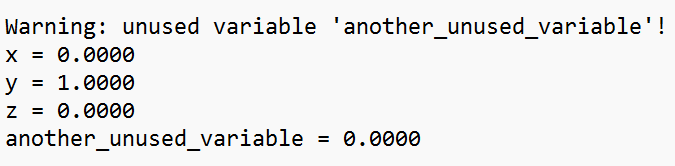
\includegraphics[width=0.7\linewidth]{Dokumentace/vysledky.png}
    \caption{Grafický výstup programu}
    \label{fig:enter-label}
\end{figure}


\chapter{Závěr}
I přes všechny slepé cesty, a že jsem se po nich s nadšením vydal, se mi podařilo naprogramovat aplikaci, která splňuje požadavky zadání.

Projekt byl otestován notebooku HP ProBook s 8GB RAM a 1.6 GHz, program se ukázal jako velmi rychlý, kdy i pro větší počet proměnných dokončil výpočty čase okolo jedné sekundy.

\begin{table}[h!]
\centering
\begin{tabular}{|>{\centering\arraybackslash}p{3cm}|>{\centering\arraybackslash}p{3cm}|>{\centering\arraybackslash}p{3cm}|}
\hline
\textbf{Čas [s]} & \textbf{Proměnné [n]} & \textbf{Rovnice [n]} \\ \hline
0.003 & 2 & 2 \\ \hline
0.007 & 2 & 3 \\ \hline
0.840 & 3 & 3 \\ \hline
0.044 & 4 & 4 \\ \hline
0.090 & 4 & 6 \\ \hline
\end{tabular}
\caption{Délka běhu programu}
\end{table}

Čas běhu programu je více ovlivněn složitostí zadaných matematických výrazů než počtem proměnných či rovnic. V případě č. 3 bylo použito rovnic s vícero závorkami. Vyhodnocení těchto výrazů je slabým místem programu a zároveň kandidátem na další vylepšení.

Samotný simplexový algoritmus je velmi rychlý.

\chapter{Zdroje}
\subsubsection{Internetové zdroje}
Ryjáček, J. (2025). TGD2: Teoretické základy operačního výzkumu. Západočeská univerzita. Dostupné z:
\url{http://najada.fav.zcu.cz/~ryjacek/students/ps/TGD2.pdf},
\newline
Wikipedia contributors. (2025). Simplex algorithm. Wikipedia. Dostupné z: \url{https://en.wikipedia.org/wiki/Simplex_algorithm},
\newline
Kckurzy.cz. (2025). Kckurzy.cz (simplexová tabulka, operační výzkum) [Video]. YouTube. Dostupné z:  
\url{https://www.youtube.com/watch?v=wubr8nbi8AI}.



\chapter{Seznam vyobrazení}
\subsubsection{Tabulky}
\newline Tabulka 5.1: Délka běhu programu, vlasní vyobrazení.
\subsubsection{Obrázky}
\newline Obrázek 4.1: Grafický výstup programu, výstup z aplikace \texttt{lp.exe}.


\end{document}